\documentclass[a4paper,12pt]{report}
\usepackage{algorithmic}
\usepackage[linesnumbered,ruled,vlined]{algorithm2e}
\usepackage[margin=2cm]{geometry}
\usepackage[utf8]{inputenc}
\usepackage{listings} 
\usepackage{graphicx} 
\usepackage{color}
\usepackage{xcolor}
\usepackage{hyperref}
\usepackage{xurl}
\usepackage{pythonhighlight}
\usepackage{enumitem}

\makeatletter
\renewcommand*\contentsname{Cuprins}
\renewcommand{\@chapapp}{Capitolul}
\makeatother

\begin{document}
\vspace{-5cm}
\begin{center}
Department of Computer Science\\
Technical University of Cluj-Napoca\\

\includegraphics[width=10cm]{fig/footer}
\end{center}
\vspace{1cm}
%\maketitle
\begin{center}
\begin{Large}
\textbf{Sisteme Expert}\\
\end{Large}
\textit{Laborator 2022-2023}\\
\vspace{3cm}
\textbf{Incadrarea pe banda}\\
Proiect\\
%Tool: \\
\vspace{1.5cm}
Student: Blaj Sergiu-Emanuel\\
Grupa: 30643\\
\vspace{6cm}
Prof. Radu Razvan Slavescu\\
\vspace{1cm}

\includegraphics[width=10cm]{fig/footer}
\end{center}

\tableofcontents

%\input{policy}

\newpage

\chapter{Sensul giratoriu}

\begin{center}
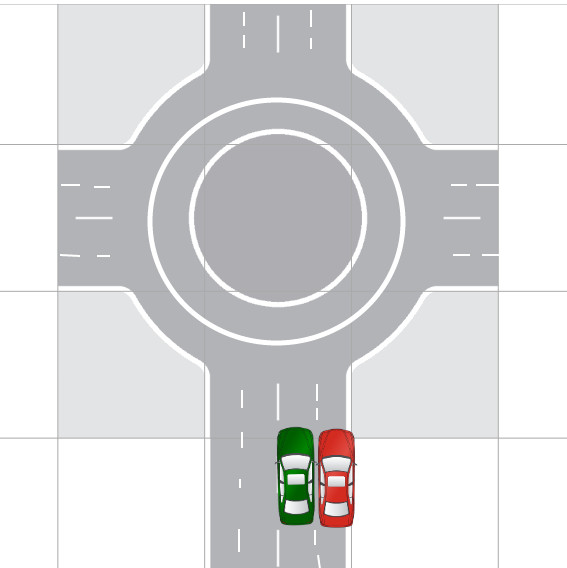
\includegraphics[width=10cm]{fig/scenariul1}
\end{center}
\begin{center}
Incadrarea pe banda in sensul giratoriu
\end{center}

\section{Descrierea scenariului}
Primul scenariu surprinde doua masini aproape de intrarea in sensul giratoriu. Ambele vehicule motorizate doresc sa faca dreapta, adica sa iasa la prima iesire din sensul giratoriu. Vehiculul verde reprezinta 'ego'-ul, iar vehiculul rosu reprezinta 'obstacolul'. Intentia a fost ca fiecare directie a drumului sa aiba doua benzi, insa, din cauza instrumentului de desen, acest lucru n-a fost posibil. \\
Aceasta situatie este o situatie destul de des intalnita in trafic, in care vehiculul verde are doua posibilitati: fie asteapta dupa vehiculul rosu pentru a se incadra pe banda de a face dreapta (scenariu pe care-l vom trata in urmatorul caz), fie patrunde in sensul giratoriu, face inconjurul lui pe banda 2 si paraseste snesul giratoriu 'la a 5-a iesire' (scenariu pe care-l tratam acum). \\
Acest scenariu trebuie tratat, deoarece, in opinia mea, un vehicul autonom ar risca sa blocheze traficul daca ar alege sa abordeze prima varianta. \\

\section{Perceptii}
Mai jos, vom prezenta perceptiile care joaca rol important in luarea deciziei: \\
\begin{itemize}
    \item flash (left OR right) - invalid daca valoarea e 'left': semnalizarea ar fi invalida;
    \item obstacle to right (true OR false) - invalid daca e 'true': vehiculul n-ar avea spatiu sa vireze dreapta;
    \item distance - invalid daca e mai mica decat '25': nu se pot executa manevre la mai putin de 25 metri de sensul giratoriu, treceri de pietoni, etc.;
    \item direction (left, ahead OR right) - invalid daca e 'left': nu se poate vira la dreapta, daca directia de conducere e stanga.
\end{itemize}

\section{Output}
AGENT roundabout-framing-maneuver = agentul care verifica manevra de incadrare pe banda in sensul giratoriu: \\
\begin{itemize}
    \item prohibited - manevra interzisa
    \item allowed - manevra permisa
\end{itemize}
PERCEPT-MANAGER: timp = 1 \\
\rule{1cm} *AGENT roundabout-framing-maneuver prohibited \\
 PERCEPT-MANAGER: timp = 2 \\
\rule{1cm} *AGENT roundabout-framing-maneuver prohibited \\
. . . \\
 PERCEPT-MANAGER: timp = 23 \\
\rule{1cm} *AGENT roundabout-framing-maneuver prohibited \\
PERCEPT-MANAGER: timp = 24 \\
\rule{1cm} *AGENT roundabout-framing-maneuver allowed \\
PERCEPT-MANAGER: timp = 25 \\
\rule{1cm} *AGENT roundabout-framing-maneuver allowed \\
PERCEPT-MANAGER: timp = 26 \\
\rule{1cm} *AGENT roundabout-framing-maneuver allowed \\

\newpage

\section{Timpi}
Fiecare pas din agent a fost supus unor masuratori (5 la numar). Pentru primii 3 pasi, tabelul cu date arata in felul urmator:\\

\begin{center}
\begin{data_table}
\begin{tabular}{||c c c c||} 
 \hline
nr & timp (s) & \mu (media) (s) & \sigma (deviatia) (s)\\
 \hline
1 & 0.000250101 & & \\
2 & 0.000173807 & & \\
3 & 0.000198347 & 0.000204026 & 0.000002652 \\
4 & 0.000212980 & & \\
5 & 0.000184895 & & \\
\hline
\end{tabular}
\end{data_table}
\end{center}
\begin{center}
Timpii pentru inferenta sensului giratoriu la t = 1
\end{center}

\begin{center}
\begin{data_table}
\begin{tabular}{||c c c c||} 
 \hline
nr & timp (s) & \mu (media) (s) & \sigma (deviatia) (s)\\
 \hline
1 & 0.000273268 & & \\
2 & 0.000214145 & & \\
3 & 0.000230294 & 0.000244674 & 0.000003827 \\
4 & 0.000269486 & & \\
5 & 0.000260654 & & \\
\hline
\end{tabular}
\end{data_table}
\end{center}
\begin{center}
Timpii pentru inferenta sensului giratoriu la t = 2
\end{center}

\begin{center}
\begin{data_table}
\begin{tabular}{||c c c c||} 
 \hline
nr & timp (s) & \mu (media) (s) & \sigma (deviatia) (s)\\
 \hline
1 & 0.000158932 & & \\
2 & 0.000193593 & & \\
3 & 0.000129519 & 0.000224081 & 0.000008466 \\
4 & 0.000294925 & & \\
5 & 0.000212041 & & \\
\hline
\end{tabular}
\end{data_table}
\end{center}
\begin{center}
Timpii pentru inferenta sensului giratoriu la t = 3
\end{center}

\newpage

\chapter{Intersectie}

\begin{center}
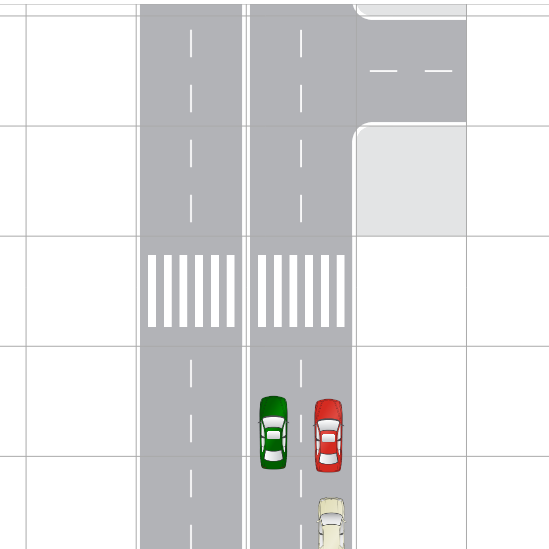
\includegraphics[width=10cm]{fig/scenariul2}
\end{center}
\begin{center}
Incadrarea inaintea unei intersectii
\end{center}

\section{Descrierea scenariului}
Al doilea scenariu surprinde trei masini aproape de o intersectie, inaintea careia se afla o trecere de pietoni. Vehiculul verde reprezinta 'ego'-ul, iar vehiculul rosu reprezinta 'obstacolul'. Ego-ul doreste sa opreasca la un magazin situat langa banda 1, dupa trecerea de pietoni, dar inainte de intersectie. \\
Aceasta situatie este o situatie destul de des intalnita in trafic, in care vehiculul verde are doua posibilitati: fie renunta la popasul sau, fie asteapta dupa vehiculul rosu pentru a se incadra pe banda de a face dreapta (scenariu pe care-l vom trata acum).\\
Acest scenariu trebuie tratat, deoarece, in opinia mea, un vehicul autonom ar cauta o reconfigurare a rutei, consumand mai mult combustibil si energie. Eventualii pietoni pe trecerea de pietoni nu ar influenta, deoarece manevra se va executa cu cel putin 25 de metri inainte de aceasta. \\

\section{Perceptii}
Mai jos, vom prezenta perceptiile care joaca rol important in luarea deciziei: \\
\begin{itemize}
    \item flash (left OR right) - invalid daca valoarea e 'left': semnalizarea ar fi invalida;
    \item obstacle to right (true OR false) - invalid daca e 'true': vehiculul n-ar avea spatiu sa vireze dreapta;
    \item distance - invalid daca e mai mica decat '25': nu se pot executa manevre la mai putin de 25 metri de sensul giratoriu, treceri de pietoni, etc.;
    \item direction (left, ahead OR right) - invalid daca e 'left': nu se poate vira la dreapta, daca directia de conducere e stanga.
\end{itemize}

\section{Output}
AGENT intersection-framing-maneuver = agentul care verifica manevra de incadrare pe banda in intersectie: \\
\begin{itemize}
    \item prohibited - manevra interzisa
    \item allowed - manevra permisa
\end{itemize}
PERCEPT-MANAGER: timp = 1 \\
\rule{1cm} *AGENT intersection-framing-maneuver prohibited \\
 PERCEPT-MANAGER: timp = 2 \\
\rule{1cm} *AGENT intersection-framing-maneuver prohibited \\
PERCEPT-MANAGER: timp = 3 \\
\rule{1cm} *AGENT intersection-framing-maneuver prohibited \\
PERCEPT-MANAGER: timp = 4 \\
\rule{1cm} *AGENT intersection-framing-maneuver prohibited \\
PERCEPT-MANAGER: timp = 5 \\
\rule{1cm} *AGENT intersection-framing-maneuver prohibited \\
PERCEPT-MANAGER: timp = 6 \\
\rule{1cm} *AGENT intersection-framing-maneuver prohibited \\
PERCEPT-MANAGER: timp = 7 \\
\rule{1cm} *AGENT intersection-framing-maneuver allowed \\
PERCEPT-MANAGER: timp = 8 \\
\rule{1cm} *AGENT intersection-framing-maneuver prohibited \\
PERCEPT-MANAGER: timp = 9 \\
\rule{1cm} *AGENT intersection-framing-maneuver prohibited \\

\newpage

\section{Timpi}
Fiecare pas din agent a fost supus unor masuratori (5 la numar). Pentru primii 3 pasi, tabelul cu date arata in felul urmator:\\

\begin{center}
\begin{data_table}
\begin{tabular}{||c c c c||} 
 \hline
nr & timp (s) & \mu (media) (s) & \sigma (deviatia) (s)\\
 \hline
1 & 0.000607345 & & \\
2 & 0.000597382 & & \\
3 & 0.000599784 & 0.000541205 & 0.000003901 \\
4 & 0.000491284 & & \\
5 & 0.000610953 & & \\
\hline
\end{tabular}
\end{data_table}
\end{center}
\begin{center}
Timpii pentru inferenta intersectiei la t = 1
\end{center}

\begin{center}
\begin{data_table}
\begin{tabular}{||c c c c||} 
 \hline
nr & timp (s) & \mu (media) (s) & \sigma (deviatia) (s)\\
 \hline
1 & 0.000705921 & & \\
2 & 0.000699520 & & \\
3 & 0.000650349 & 0.000669785 & 0.000003958 \\
4 & 0.000640291 & & \\
5 & 0.000685496 & & \\
\hline
\end{tabular}
\end{data_table}
\end{center}
\begin{center}
Timpii pentru inferenta intersectiei la t = 2
\end{center}

\begin{center}
\begin{data_table}
\begin{tabular}{||c c c c||} 
 \hline
nr & timp (s) & \mu (media) (s) & \sigma (deviatia) (s)\\
 \hline
1 & 0.000694830 & & \\
2 & 0.000609732 & & \\
3 & 0.000659531 & 0.000647285 & 0.00004524 \\
4 & 0.000695024 & & \\
5 & 0.000651238 & & \\
\hline
\end{tabular}
\end{data_table}
\end{center}
\begin{center}
Timpii pentru inferenta intersectiei la t = 3
\end{center}

\begin{center}
\begin{data_table}
\begin{tabular}{||c c c c||} 
 \hline
nr & timp (s) & \mu (media) (s) & \sigma (deviatia) (s)\\
 \hline
1 & 0.000354352 & & \\
2 & 0.000342915 & & \\
3 & 0.000329242 & 0.000320078 & 0.000010242 \\
4 & 0.000310532 & & \\
5 & 0.000296432 & & \\
\hline
\end{tabular}
\end{data_table}
\end{center}
\begin{center}
Timpii pentru inferenta intersectiei la t = 4
\end{center}

\begin{center}
\begin{data_table}
\begin{tabular}{||c c c c||} 
 \hline
nr & timp (s) & \mu (media) (s) & \sigma (deviatia) (s)\\
 \hline
1 & 0.000302552 & & \\
2 & 0.000298912 & & \\
3 & 0.000319630 & 0.000301521 & 0.000002442 \\
4 & 0.000320602 & & \\
5 & 0.000290012 & & \\
\hline
\end{tabular}
\end{data_table}
\end{center}
\begin{center}
Timpii pentru inferenta intersectiei la t = 5
\end{center}

\begin{center}
\begin{data_table}
\begin{tabular}{||c c c c||} 
 \hline
nr & timp (s) & \mu (media) (s) & \sigma (deviatia) (s)\\
 \hline
1 & 0.000251252 & & \\
2 & 0.000235912 & & \\
3 & 0.000241630 & 0.000269032 & 0.000005302 \\
4 & 0.000270602 & & \\
5 & 0.000287012 & & \\
\hline
\end{tabular}
\end{data_table}
\end{center}
\begin{center}
Timpii pentru inferenta intersectiei la t = 6
\end{center}

\begin{center}
\begin{data_table}
\begin{tabular}{||c c c c||} 
 \hline
nr & timp (s) & \mu (media) (s) & \sigma (deviatia) (s)\\
 \hline
1 & 0.000363052 & & \\
2 & 0.000348912 & & \\
3 & 0.000349530 & 0.000349865 & 0.000001957 \\
4 & 0.000320602 & & \\
5 & 0.000340512 & & \\
\hline
\end{tabular}
\end{data_table}
\end{center}
\begin{center}
Timpii pentru inferenta intersectiei la t = 7
\end{center}

\begin{center}
\begin{data_table}
\begin{tabular}{||c c c c||} 
 \hline
nr & timp (s) & \mu (media) (s) & \sigma (deviatia) (s)\\
 \hline
1 & 0.000138052 & & \\
2 & 0.000186912 & & \\
3 & 0.000197630 & 0.000163125 & 0.000008692 \\
4 & 0.000147602 & & \\
5 & 0.000155012 & & \\
\hline
\end{tabular}
\end{data_table}
\end{center}
\begin{center}
Timpii pentru inferenta intersectiei la t = 8
\end{center}

\begin{center}
\begin{data_table}
\begin{tabular}{||c c c c||} 
 \hline
nr & timp (s) & \mu (media) (s) & \sigma (deviatia) (s)\\
 \hline
1 & 0.000126052 & & \\
2 & 0.000104912 & & \\
3 & 0.000113630 & 0.000120912 & 0.000004021 \\
4 & 0.000135602 & & \\
5 & 0.000120912 & & \\
\hline
\end{tabular}
\end{data_table}
\end{center}
\begin{center}
Timpii pentru inferenta intersectiei la t = 9
\end{center}

\newpage


\chapter{Autostrada}

\begin{center}
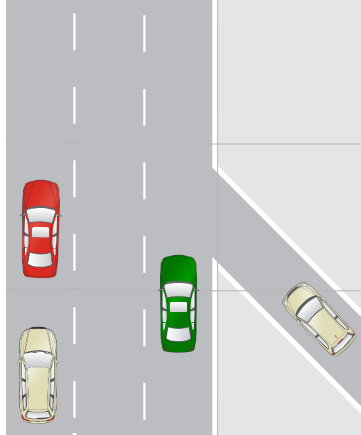
\includegraphics[width=10cm]{fig/scenariul3}
\end{center}
\begin{center}
Incadrarea pe autostrada
\end{center}

\section{Descrierea scenariului}
Ultimul, dar nu cel din urma scenariu, surprinde cateva masini aflate pe o autostrada. Toate vehicule motorizate doresc sa se incadreze pe banda 2 (banda din mijloc). Vehiculul verde reprezinta 'ego'-ul, iar vehiculele rosu si alb reprezinta 'obstacolele'. \\
Aceasta situatie este o situatie destul de des intalnita in trafic, in care vehiculul verde are doua posibilitati: fie asteapta dupa vehiculele rosu si alb pentru a se incadra pe bada, fie isi reconfigureaza ruta.\\
Acest scenariu trebuie tratat, deoarece, in opinia mea, un vehicul autonom ar risca sa provoace un accident, daca n-ar sti ca el trebuie sa cedeze prioritatea.\\

\section{Output}
AGENT highway-framing-maneuver = agentul care verifica manevra de incadrare pe banda pe autostrada: \\
\begin{itemize}
    \item prohibited - manevra interzisa
    \item allowed - manevra permisa
\end{itemize}
PERCEPT-MANAGER: timp = 1\\
\rule{1cm} *AGENT highway-framing-maneuver prohibited\\
PERCEPT-MANAGER: timp = 2\\
\rule{1cm} *AGENT highway-framing-maneuver prohibited\\
PERCEPT-MANAGER: timp = 3\\
\rule{1cm} *AGENT highway-framing-maneuver prohibited\\
PERCEPT-MANAGER: timp = 4\\
\rule{1cm} *AGENT highway-framing-maneuver prohibited\\
PERCEPT-MANAGER: timp = 5\\
\rule{1cm} *AGENT highway-framing-maneuver prohibited\\
PERCEPT-MANAGER: timp = 6\\
\rule{1cm} *AGENT highway-framing-maneuver allowed\\
PERCEPT-MANAGER: timp = 7\\
\rule{1cm} *AGENT highway-framing-maneuver allowed\\

\section{Perceptii}
Mai jos, vom prezenta perceptiile care joaca rol important in luarea deciziei: \\
\begin{itemize}
    \item ego-flash (left OR right) - invalid daca valoarea e 'right': semnalizarea ar fi invalida, ego-ul fiind nevoit sa semnalizeze stanga;
    \item opponent-flash (left OR right) - invalid daca valoarea e 'right': cei de pe banda 3 au prioritate fata de cei de pe banda 1 la schimbarea pe banda 2;
    \item obstacle to left (true OR false) - invalid daca e 'true': vehiculul n-ar avea spatiu sa vireze stanga;
    \item direction (left, ahead OR right) - invalid daca e 'right': nu se poate vira la stanga, daca directia de conducere e dreapta.
\end{itemize}

\newpage

\section{Timpi}
Fiecare pas din agent a fost supus unor masuratori (5 la numar). Pentru primii 3 pasi, tabelul cu date arata in felul urmator:\\

\begin{center}
\begin{data_table}
\begin{tabular}{||c c c c||} 
 \hline
nr & timp (s) & \mu (media) (s) & \sigma (deviatia) (s)\\
 \hline
1 & 0.000310129 & & \\
2 & 0.000329451 & & \\
3 & 0.000291248 & 0.000310986 & 0.000000792 \\
4 & 0.000295329 & & \\
5 & 0.000319294 & & \\
\hline
\end{tabular}
\end{data_table}
\end{center}
\begin{center}
Timpii pentru inferenta autostrazii la t = 1
\end{center}

\begin{center}
\begin{data_table}
\begin{tabular}{||c c c c||} 
 \hline
nr & timp (s) & \mu (media) (s) & \sigma (deviatia) (s)\\
 \hline
1 & 0.000312052 & & \\
2 & 0.000290125 & & \\
3 & 0.000301230 & 0.000301205 & 0.000000958 \\
4 & 0.000310502 & & \\
5 & 0.000290012 & & \\
\hline
\end{tabular}
\end{data_table}
\end{center}
\begin{center}
Timpii pentru inferenta autostrazii la t = 2
\end{center}

\begin{center}
\begin{data_table}
\begin{tabular}{||c c c c||} 
 \hline
nr & timp (s) & \mu (media) (s) & \sigma (deviatia) (s)\\
 \hline
1 & 0.000363052 & & \\
2 & 0.000298912 & & \\
3 & 0.000329630 & 0.000301205 & 0.000000768 \\
4 & 0.000310602 & & \\
5 & 0.000290012 & & \\
\hline
\end{tabular}
\end{data_table}
\end{center}
\begin{center}
Timpii pentru inferenta autostrazii la t = 3
\end{center}

\begin{center}
\begin{data_table}
\begin{tabular}{||c c c c||} 
 \hline
nr & timp (s) & \mu (media) (s) & \sigma (deviatia) (s)\\
 \hline
1 & 0.000264985 & & \\
2 & 0.000298912 & & \\
3 & 0.000323124 & 0.000282918 & 0.00008219 \\
4 & 0.000290128 & & \\
5 & 0.000290012 & & \\
\hline
\end{tabular}
\end{data_table}
\end{center}
\begin{center}
Timpii pentru inferenta autostrazii la t = 4
\end{center}

\begin{center}
\begin{data_table}
\begin{tabular}{||c c c c||} 
 \hline
nr & timp (s) & \mu (media) (s) & \sigma (deviatia) (s)\\
 \hline
1 & 0.000413298 & & \\
2 & 0.000492152 & & \\
3 & 0.000459325 & 0.000434831 & 0.000009125 \\
4 & 0.000392018 & & \\
5 & 0.000482195 & & \\
\hline
\end{tabular}
\end{data_table}
\end{center}
\begin{center}
Timpii pentru inferenta autostrazii la t = 5
\end{center}

\begin{center}
\begin{data_table}
\begin{tabular}{||c c c c||} 
 \hline
nr & timp (s) & \mu (media) (s) & \sigma (deviatia) (s)\\
 \hline
1 & 0.000361525 & & \\
2 & 0.000330214 & & \\
3 & 0.000329232 & 0.000323242 & 0.000005768 \\
4 & 0.000310602 & & \\
5 & 0.000290012 & & \\
\hline
\end{tabular}
\end{data_table}
\end{center}
\begin{center}
Timpii pentru inferenta autostrazii la t = 6
\end{center}

\begin{center}
\begin{data_table}
\begin{tabular}{||c c c c||} 
 \hline
nr & timp (s) & \mu (media) (s) & \sigma (deviatia) (s)\\
 \hline
1 & 0.000150204 & & \\
2 & 0.000201092 & & \\
3 & 0.000176948 & 0.000182059 & 0.000006768 \\
4 & 0.000195029 & & \\
5 & 0.000202523 & & \\
\hline
\end{tabular}
\end{data_table}
\end{center}
\begin{center}
Timpii pentru inferenta autostrazii la t = 7
\end{center}

\newpage

\chapter{Anexa}
Agentul a fost rulat pe urmatorul build: \\
\rule{1cm}* CPU: Intel\textcopyright Core\textregistered i7-8565U Processor (8M Cache, up to 4.60 GHz), 4 cores, 8 threads \\
\rule{1cm}* GPU: nVidia GeForce MX230 2GB \\
\rule{1cm}* RAM: 12GB @ 2400MHz \\
\rule{1cm}* OS: Ubuntu 20.04.5 LTS, x64 \\
\\
Articole folositoare: \\
\begin{itemize}
    \item Detectarea directiei masinii (pentru perceptia 'direction'): \\ \href{https://www.freepatentsonline.com/6141605.html}{Determining the direction of travel of an automotive vehicle from yaw rate and relative steering wheel angle} 
    \item Detectarea spatiului liber din jurul masinii (pentru perceptia 'obstacle'): \\
    \href{https://www.mdpi.com/1424-8220/22/1/315}{Free Space Detection Algorithm Using Object Tracking for Autonomous Vehicles}
    \item Detectarea trecerii de pietoni, a sensului giratoriu (pentru perceptia 'distance'): \\
    \href{https://koasas.kaist.ac.kr/bitstream/10203/259082/1/75167.pdf}{Crosswalk and Traffic Light Detection via Integral Framework}
\end{itemize}

\end{document}

